\documentclass[a4paper,8pt,twocolumn,twoside,]{pinp}

%% Some pieces required from the pandoc template
\providecommand{\tightlist}{%
  \setlength{\itemsep}{0pt}\setlength{\parskip}{0pt}}

% Use the lineno option to display guide line numbers if required.
% Note that the use of elements such as single-column equations
% may affect the guide line number alignment.

\usepackage[T1]{fontenc}
\usepackage[utf8]{inputenc}

% pinp change: the geometry package layout settings need to be set here, not in pinp.cls
\geometry{layoutsize={0.95588\paperwidth,0.98864\paperheight},%
  layouthoffset=0.02206\paperwidth, layoutvoffset=0.00568\paperheight}

\definecolor{pinpblue}{HTML}{185FAF}  % imagecolorpicker on blue for new R logo
\definecolor{pnasbluetext}{RGB}{101,0,0} %



\title{Analysing Student Performance - Portuguese Language Class}

\author[]{smck0583, mcza2974, ttie8223, dpha3771, kmao8943}


\setcounter{secnumdepth}{0}

% Please give the surname of the lead author for the running footer
\leadauthor{}

% Keywords are not mandatory, but authors are strongly encouraged to provide them. If provided, please include two to five keywords, separated by the pipe symbol, e.g:
 

\begin{abstract}

\end{abstract}

\dates{Git Repository -
\url{https://github.sydney.edu.au/smck0583/CC05E4}}


% initially we use doi so keep for backwards compatibility
% new name is doi_footer


\begin{document}

% Optional adjustment to line up main text (after abstract) of first page with line numbers, when using both lineno and twocolumn options.
% You should only change this length when you've finalised the article contents.
\verticaladjustment{-2pt}

\maketitle
\thispagestyle{firststyle}
\ifthenelse{\boolean{shortarticle}}{\ifthenelse{\boolean{singlecolumn}}{\abscontentformatted}{\abscontent}}{}

% If your first paragraph (i.e. with the \dropcap) contains a list environment (quote, quotation, theorem, definition, enumerate, itemize...), the line after the list may have some extra indentation. If this is the case, add \parshape=0 to the end of the list environment.


List of packages used:
\href{https://cran.r-project.org/package=ggplot2}{ggplot2}\cite{CRAN:ggplot2}
\href{https://cran.r-project.org/package=dplyr}{dplyr}
\href{https://cran.r-project.org/package=olsrr}{olsrr}
\href{https://cran.r-project.org/package=pinp}{pinp}
\href{https://cran.r-project.org/package=tinytex}{tinytex}\citep{CRAN:tinytex}
\href{https://cran.r-project.org/package=tidyverse}{tidyverse}\citep{CRAN:tidyverse}
\href{https://cran.r-project.org/package=stargazer}{stargazer}\citep{CRAN:stargazer}
Data source: \citet{art:UCI}

\hypertarget{abstract}{%
\subsection{Abstract}\label{abstract}}

This report investigates the effect of various attributes on final grade
in Portuguese language class from data of 649 secondary students in
Portugal, and aims to use multiple linear regression to produce a model
that closely predicts final grade in Portuguese for students in
Portuguese public secondary schools. The dataset contains 32 attributes
school-related, demographic, lifestyle and socioeconomic factors. The
final model was chosen by AIC in a stepwise algorithm and has an RMSE of
0.84 and an R-squared value of 0.90. The predictor variables are first
period grade, second period grade, student age, number of previous class
failures, degree of workday alcohol consumption, desire to pursue higher
education, presence of extra educational support, health status, and
degree of going out with friends.

\hypertarget{introduction}{%
\subsection{Introduction}\label{introduction}}

Portuguese ability level plays a significant role in the lives of people
living in Portugal, thus it is important to provide early support to
students who perform poorly in Portuguese relative to their peers before
the variance of ability levels between students compound. However, most
Portuguese public schools store student data such as school reports on
physical paper rather than digitally, which makes it difficult to track
student scores. Thus, an alternative strategy to provide early support
to students would be to direct additional resources to students that are
predicted to perform poorly in Portuguese. This report explores the
questions: What factors have significant impacts on final Portuguese
grades for students in Portuguese public secondary schools? What
category of the variables was most prominent? The results of the
resulting investigations can help predict which students will require
additional Portuguese support and help improve education outcomes.

\hypertarget{data-set-description}{%
\subsection{Data Set Description}\label{data-set-description}}

This report uses student data collected by Paulo Cortez and Alice Silva
(University of Minho, 2005-2006) from 649 students across two Portuguese
public secondary schools. The dataset consists of 33 attributes and was
formed by combining data from school reports, which contained student
grades and number of absences, and from questionnaire responses, which
consisted of demographic, lifestyle and socioeconomic variables that
were predicted to impact student performance. More specifically, the
dataset contains 3 attributes which are related to student grade, namely
G1, G2, and G3, which are values between 0 and 20 representing the first
period grade, second period grade, and final grade respectively.

\hypertarget{analysis}{%
\subsection{Analysis}\label{analysis}}

\hypertarget{full-model-assumption-checking}{%
\subsubsection{Full Model Assumption
Checking}\label{full-model-assumption-checking}}

The initial model applied to the data set was a full linear model
constructed from all of the variables on the untouched data set.
Importantly, the assumptions of the underlying model seemingly weren't
sufficiently met when initially inspected. Both homoscedasticity and
normality of residuals assumptions were not upheld, the best example of
this is shown in figure-\ref{fig:FR} which features heteroscedastic
placement of residuals in the lower left hand quadrant of the figure.

\begin{figure}

{\centering 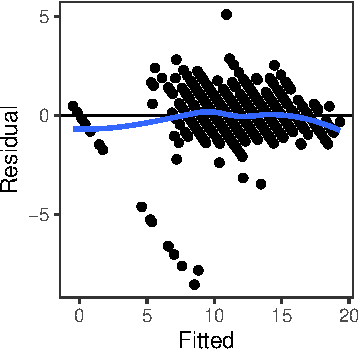
\includegraphics{CC05E4-FinalReport_files/figure-latex/FR-1} 

}

\caption{Residual Plot of the Full Model}\label{fig:FR}
\end{figure}

After inspection these heteroscedastic data points correspond to zero
scoring students in the final exams (G3 = 0), this is indicative of
students who were absent or got caught cheating on their final exam, as
this result differs from the aim of this investigation they shall be
removed from further analysis. Additionally two outliers were detected
using Cook's Distance in figure-\ref{fig:outlier} and so were removed to
reduce their effect on the final model.

\hypertarget{derivation-of-final-model}{%
\subsubsection{Derivation of Final
Model}\label{derivation-of-final-model}}

The data set has now been transformed to fit the assumptions of the
linear model, however, in order to derive an optimal model, forward and
backward AIC and BIC model derivations may be used. The optimal model
was found to be the forward AIC model as this model outperformed both
the full baseline model but also forward and backward BIC models in
terms of coefficient of determination (noting that both AIC and BIC
forward and backward models had identical results)
(figure-\ref{fig:aicdev}) (equation-\ref{eqn:example}). With AIC
deriving an adjusted coefficient of determination of 0.909 and AIC score
of 1524.877, hence the forward AIC model will be selected as the final
model (table-\ref{tab:tablefin}).

\begin{equation}
  \begin{aligned}
       G3 = -0.586 + 0.741\text{G2} + 0.199\text{G1} + 0.119\text{age} \\
       - 0.173\text{failures} - 0.091\text{Dalc} + 0.310\text{higher[yes]} \\
       - 0.236\text{schoolsup[yes]} - 0.047\text{health } - 0.044\text{goout} \\
       \label{eqn:example} 
  \end{aligned}
\end{equation}

\begin{figure}

{\centering 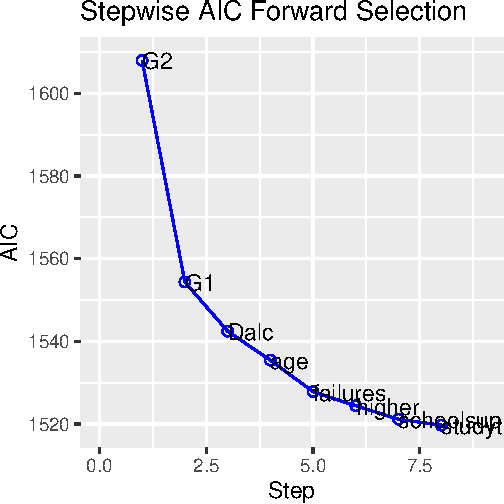
\includegraphics{CC05E4-FinalReport_files/figure-latex/aicdev-1} 

}

\caption{AIC Optimzed Model Derivation}\label{fig:aicdev}
\end{figure}

\hypertarget{final-model-assumptions}{%
\subsubsection{Final Model Assumptions}\label{final-model-assumptions}}

Unlike the first full model, the final model seems to satisfy the
assumptions of the linear model. The assumption of independence is
upheld given the fact that G3 is a test score and each student performed
the final test strictly independently (otherwise receiving a score of
0). Homoscedasticity was assessed with the use of a residual plot shown
in figure-\ref{fig:finres}, wherein the points seem to be evenly
scattered above and below the identity line indicating homoscedasticity.
Linearity was also assessed with the residual plot, wherein the points
are relatively flat across the fitted values this is further supported
by a relatively flat Loess fitted line indicating linearity. Normally
distributed residuals were assessed through a QQ-plot in
figure-\ref{fig:qqres}, featuring data points closely straddling the
line across the quantile range supporting the normality assumption.

\begin{figure}

{\centering 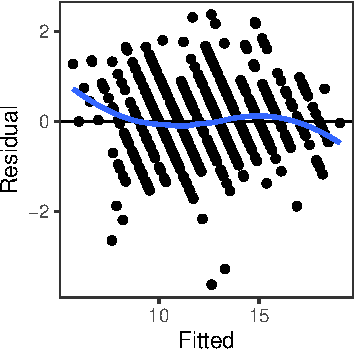
\includegraphics{CC05E4-FinalReport_files/figure-latex/finres-1} 

}

\caption{Residual Plot of Final Model}\label{fig:finres}
\end{figure}

\begin{figure}

{\centering 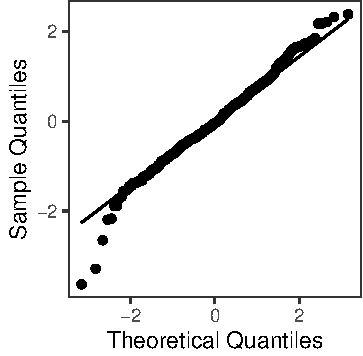
\includegraphics{CC05E4-FinalReport_files/figure-latex/qqres-1} 

}

\caption{QQ-Plot of Final Model}\label{fig:qqres}
\end{figure}

\hypertarget{results}{%
\subsection{Results}\label{results}}

The final linear model is shown above (\ref{eqn:example}). Here it is
interesting to note that the AIC fell from 1579.18 in the backward model
and 1578.6 in the forward model to 1524.877 and 1524.877 respectively,
in the final model. Indicating the final model is a better model as a
result of the lower AIC. This also the case with the BIC falling from
1581.603 in both forward and backward, and in the final BIC being
1533.832. Furthermore, in the original AIC model the adjusted r\^{}2 for
the forward model was 0.901 and 0.902 in the backward model, whereas in
the final model, the adjusted R\^{}2 was 0.909 and 0.909 respectively,
indicating the final better fit the data, this was mostly likely due to
the removal of outliers. This is also the case with the BIC model with
the r\^{}2 increasing from 0.900 (in both forward and back) to 0.907 (
again in both), indicating the BIC model improved as well in the final
model.

\hypertarget{discussion-and-limitations}{%
\subsection{Discussion and
Limitations}\label{discussion-and-limitations}}

In answering our key questions, the variables found to predict student
performance from the forward AIC model were first period grade, second
period grade, age, number of past class failures, average workday
alcohol consumption, whether students want to take higher education, if
they have extra educational support, current health status and how often
they go out with friends. Categorising these under demographic,
lifestyle and school related variables as outlined in Cortex and Silva
(2008), we infer lifestyle and school related variables to equally
contribute to predicting student achievement. Considering first and
second period grades are well correlated with third period grades, to
explore other relevant factors that influence student performance, these
were not included in the three categories.

A limitation of this report is that there are a large number of
parameters (32) relative to the sample size (632 after pre-processing),
which makes it harder to determine whether factors have a significant
impact on the response variable. A potential improvement would be to
reduce the number of parameters in the pre-processing step by
eliminating one of the factors for any pairs of factors that are
correlated.

A further limitation is the dataset wasn't from a random sample of
Portuguese secondary school students. We already observed that there may
be a significant difference between average final scores of students in
different schools, such as between MS and GP. Since the dataset is
limited to two schools, the model may be very inaccurate for other
public secondary schools, particularly for those with significantly
different score distributions. An improvement would be to include a
larger variety of schools so that the sample is closer to a random
population. Further, only 227 of the observations were from Mousinho da
Silveira (MS) secondary school. An analysis by Molin (2020) of the
dataset had findings that Gabriel Pereira (GP) secondary school excelled
academically compared to GP. GP had mainly urban students, the lowest
proportion of failures, highest study time and offered school support.
The discrepancy between these two schools may potentially skew the data.
In addition, cross-cultural limitations may inhibit the generalisability
of findings to other populations as this study was conducted in
Portugal; a western, educated, industrialised, rich and democratic
(WEIRD) society . Future prospects for this could include acquiring data
of schools from a multitude of countries as well as ensuring an
equivalent number of observations from different schools within the same
region. Ensuring a large sample size to account for the number of
attributes will counter the issue of overfitting. On top of this, the
inclusion of both G1 and G2 in the final model results in
multicollinearity since they are correlated (see
Appendix-\ref{fig:corr}), which may reduce the accuracy of the
coefficients and increase the standard error. To avoid this, we could
remove one of the variables before performing the model selection.

\hypertarget{conclusion}{%
\subsection{Conclusion}\label{conclusion}}

In conclusion, the report aims to identify attributes that influence
student performance in secondary school which can then be used to
improve educational outcomes. These were found to be first period grade,
second period grade, age, number of previous class failures, workday
alcohol consumption, desire to pursue higher education, extra
educational support, current health status, and degree of going out with
friends. Lifestyle and school-related factors were also found to equally
contribute to the success of students in school.

\begin{table}[!htbp] \centering 
  \caption{Appendix: AIC vs Baseline Model Comparison} 
  \label{} 
\small 
\begin{tabular}{@{\extracolsep{1pt}}lcc} 
\\[-1.8ex]\hline 
\hline \\[-1.8ex] 
 & \multicolumn{2}{c}{\textit{Dependent variable:}} \\ 
\cline{2-3} 
\\[-1.8ex] & \multicolumn{2}{c}{G3} \\ 
 & AIC Models (Forward and Back) & Full Baseline Model \\ 
\\[-1.8ex] & (1) & (2)\\ 
\hline \\[-1.8ex] 
 schoolMS &  & $-$0.198 (0.128) \\ 
  sexM &  & $-$0.123 (0.118) \\ 
  G2 & 0.741$^{***}$ (0.026) & 0.870$^{***}$ (0.035) \\ 
  G1 & 0.199$^{***}$ (0.026) & 0.129$^{***}$ (0.038) \\ 
  age & 0.119$^{***}$ (0.029) & 0.029 (0.048) \\ 
  addressU &  & 0.114 (0.123) \\ 
  famsizeLE3 &  & 0.016 (0.115) \\ 
  PstatusT &  & $-$0.097 (0.163) \\ 
  Medu &  & $-$0.092 (0.071) \\ 
  Fedu &  & 0.050 (0.065) \\ 
  Mjobhealth &  & 0.266 (0.252) \\ 
  Mjobother &  & $-$0.094 (0.142) \\ 
  Mjobservices &  & 0.173 (0.175) \\ 
  Mjobteacher &  & 0.221 (0.236) \\ 
  Fjobhealth &  & $-$0.444 (0.353) \\ 
  Fjobother &  & $-$0.338 (0.214) \\ 
  Fjobservices &  & $-$0.471$^{**}$ (0.225) \\ 
  Fjobteacher &  & $-$0.544$^{*}$ (0.316) \\ 
  reasonhome &  & $-$0.079 (0.134) \\ 
  reasonother &  & $-$0.362$^{**}$ (0.172) \\ 
  reasonreputation &  & $-$0.169 (0.140) \\ 
  guardianmother &  & $-$0.025 (0.125) \\ 
  guardianother &  & 0.217 (0.249) \\ 
  traveltime &  & 0.139$^{*}$ (0.075) \\ 
  studytime &  & 0.050 (0.066) \\ 
  failures & $-$0.173$^{***}$ (0.063) & $-$0.255$^{**}$ (0.099) \\ 
  Dalc & $-$0.091$^{**}$ (0.037) & $-$0.052 (0.072) \\ 
  Walc &  & $-$0.017 (0.056) \\ 
  higheryes & 0.310$^{***}$ (0.117) & 0.207 (0.183) \\ 
  internetyes &  & 0.085 (0.130) \\ 
  romanticyes &  & $-$0.042 (0.108) \\ 
  famrel &  & $-$0.016 (0.055) \\ 
  freetime &  & $-$0.050 (0.053) \\ 
  schoolsupyes & $-$0.236$^{**}$ (0.107) & $-$0.184 (0.173) \\ 
  famsupyes &  & 0.095 (0.107) \\ 
  paidyes &  & $-$0.192 (0.217) \\ 
  activitiesyes &  & 0.012 (0.105) \\ 
  nurseryyes &  & $-$0.096 (0.127) \\ 
  health & $-$0.047$^{**}$ (0.022) & $-$0.055 (0.036) \\ 
  absences &  & 0.014 (0.012) \\ 
  goout & $-$0.044 (0.029) & $-$0.019 (0.050) \\ 
  Constant & $-$0.586 (0.531) & 0.638 (0.964) \\ 
 \hline \\[-1.8ex] 
Observations & 632 & 649 \\ 
R$^{2}$ & 0.910 & 0.860 \\ 
Adjusted R$^{2}$ & 0.909 & 0.851 \\ 
Residual Std. Error & 0.801 (df = 622) & 1.249 (df = 607) \\ 
F Statistic & 701.120$^{***}$ (df = 9; 622) & 90.951$^{***}$ (df = 41; 607) \\ 
\hline 
\hline \\[-1.8ex] 
\textit{Note:}  & \multicolumn{2}{r}{$^{*}$p$<$0.1; $^{**}$p$<$0.05; $^{***}$p$<$0.01} \\ 
\end{tabular} 
\label{tab:tablefin}
\end{table}

\begin{figure}

{\centering 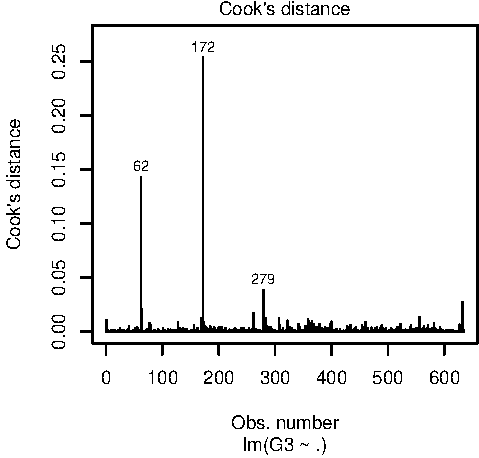
\includegraphics{CC05E4-FinalReport_files/figure-latex/outlier-1} 

}

\caption{Appendix: Cook's Distance Plot of Untouched Data Set}\label{fig:outlier}
\end{figure}

\begin{figure}

{\centering 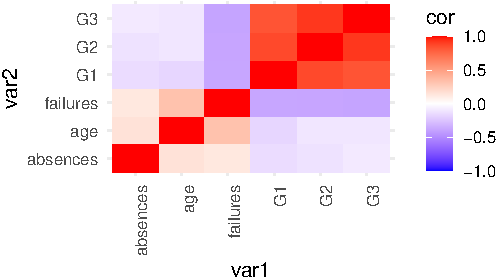
\includegraphics{CC05E4-FinalReport_files/figure-latex/corr-1} 

}

\caption{Appendix: Correlation Matrix of Numberic Variables in the Data Set}\label{fig:corr}
\end{figure}

%\showmatmethods

\pnasbreak 

\bibliography{pinp}
\bibliographystyle{jss}



\end{document}
